\documentclass[a4paper,12pt]{article}% use option titlepage to get the title on a page of its own.

\usepackage[slovene]{babel}
\usepackage[utf8]{inputenc}
\usepackage[T1]{fontenc}
\usepackage{lmodern}
\usepackage{amsmath}
\usepackage{amssymb}
\usepackage[shortlabels]{enumitem}

\usepackage{graphicx}


\title{Analiza različnih modelov trgovanja na decentraliziranih borzah \\ \large Poročilo za projekt pri predmetu Matematika z računalnikom}
\date{Maj 2024}
\author{Špela Bernardič in Nika Pavlič}

\begin{document}
\maketitle
%\section*{Plan dela}

\section*{Nekaj pojmov in pojasnil} 

\subsection*{Pametne pogodbe} 
Pametne pogodbe so digitalne pogodbe, shranjene na blockchainu, ki se samodejno izvedejo, ko so izpolnjeni vnaprej določeni pogoji.
Običajno se uporabljajo za avtomatizacijo izvajanja dogovora, tako da so lahko vsi udeleženci takoj prepričani o izidu, 
brez vpletenosti posrednika ali izgube časa. Prav tako lahko avtomatizirajo potek dela in sprožijo sledeče dejanje, 
ko so izpolnjeni vnaprej določeni pogoji.

\subsection{ERC-20 }

ERC-20 je standard za \textbf{fungible} tokene (t.j. tokeni so si med seboj popolnoma enaki (po vrsti in vrednosti)). ERC-20 token na primer deluje enako kot ETH, kar pomeni, da 1 žeton je in bo vedno enak vsem drugim žetonom.

\subsection{Impermanent loss}
\textbf{Impermanent loss} je izguba, ki jo ponudnik likvidnosti utrpi, ko zagotovi likvidnost bazenu/skladu potem pa se cene vloženih sredstev spremenijo. \textbf{Impermanent loss} se pojavi zaradi stalnega uravnovešanja likvidnostnih bazenov, kot odziv na gibanje tržnih cen. Izguba se ne realizira dokler ponudnik likvidnosti ne umakne svojih sredstev iz bazena/sklada. Če se cene tokenov vrnejo v prvotno razmerje \textbf{Impermanent loss} izgine. Ponudniki likvidnosti za zagotavljanje likvidnosti prejemajo provizije od trgovanja, ki lahko izravnajo \textbf{impermanent loss}, vendar lahko na nestabilnih trgih ali med ektremnimi gibanji cen \textbf{impermanent loss} preseže zaslužene provizije. 
% ```{r include = FALSE}
% %Izguba se realizira šele, ko ponudnik svoja sredstva umakne iz bazena/sklada. 

% # Čeprav je izguba pogosto predstavljena kot začasna, pa lahko ponudnik likvidnosti izgubo utrpi dolgoročno; npr. če je vložil dva tokena in ju je prisiljen prodati, preden se njihove cene ustalijo na prvotno razmerje. 
% # 
% # IL se pojavi zaradi stalnega uravnovešanja likvidnostnih bazenov, kot odziv na gibanje tržnih cen. 
% # 
% # Ko ponudnik likvidnosti doda tokene v sklad, običajno prispeva enako vrednost vsakega tokena v paru. Če se cena vloženih sredstev spremeni, se spremeni vrednost imetja ponudnika likvidnosti. Do **impermanent loss** pride, ko vrednost tokenov v likvidnostnem bazenu/skladu odstopa od vrednosti 
% # 
% # Izguba se ne realizira dokler ponudnik likvidnosti ne umakne svojih sredstev iz sklada. Če se cene tokenov vrnejo v prvotno razmerje IL izgine. 
% # Ponudniki likvidnosti za zagotavljanje likvidnosti prejemajo provizije od trgovanja, ki lahko izravnajo IL, vendar lahko na nestabilnih trgih ali med ekstremnimi gibanji cen IL preseže zaslužene provizije.
% ```

 

\section{Uniswap}
Uniswap največja decentralizirana borza, ki je začela delovati leta 2018. Uvedla je \textbf{automated market maker (AMM)} namesto tradicionalnih \textbf{order book}, ki jih uporabljajo borze. Deluje na Ethereum blockchainu in uporablja vrsto pametnih pogodb (ang. \textit{smart contracts}) za varno zamenjavo ERC-20 tokenov med uporabniki brez posrednika. 

Decentraliziran vidik protokola pomeni, da borze ne vodi nobena centraizirana avtoriteta. Namesto tega so zamenjave opravljene 'ena na ena ' (ang. \textit{peer to peer}). Uniswap se trudi rešiti problem likvidnosti, s katerim se srečujejo na drugih borzah. Z vsako novo verzijo Uniswap poskuša zagotoviti bolj varno, efektivno in uporabno platformo. 

% Uniswap je največja decentralizirana borza, ki deluje na Ethereum blockchainu. Uporabnikom omogoča trgovanje s kriptovalutami brez posrednika. **Uniswap pioneered the Automated Market Maker model**, kjer uporabniki **supply** Ethereum tokene v Uniswapov likvidnostni bazen algoritmi pa določijo tržno ceno na podlagi ponudbe in povpraševanja. S tem, ko uporabniki **supplayajo** tokene v likvidnostne bazene, lahko prejmejo nagrade in hkrati omogočajo **peer-to-peer** trgovanje. Kdorkoli lahko **supplya** tokene v likvidnostne bazene, z njimi trguje ali celo ustvari svoje. 





\subsection{Uniswap v2}
Uniswap V2 je izšla maja 2020. V2 je uporabnikom omogočila neposredno trgovanje s katerima koli ERC-20 tokenoma, namesto preko ETH (V1). S tem se je zmanjšalo število transakcij in prihranilo na \textbf{gas fees}. Verzija je uvedla decentraliziran cenovni orakelj, ki je ponujal zanesljive podatke o cenah v realnem času. S tem je protokol postal bolj odporen proti manipulaciji s cenami. Uvedli so tudi t.i \textbf{flash swaps}, ki so omogočile, da si uporabniki izposodijo poljubno količino tokenov iz likvidnostega \textbf{bazena/sklada??}, z njimi izvedejo želeno dejanje in v okviru iste transakcije vrnejo izposojene tokene. 

\subsubsection{Likvidnost} 
V Uniswap v2 je likvidnost enakomerno porazdeljena po cenovni krivulji $x\cdot y = k$, kjer sta x in y količina tokenov X in Y v likvidnostnem bazenu, k pa je konstanta. Likvidnost se torej zagotavlja za celotno cenovno območje $(0,\infty)$. V večini likvidnostnih bazenov, ta likvidnost ni nikoli uporabljena. 

Ponudniki likvidnosti Uniswapa V2 zaslužijo provizije le za majhen del svojega kapitala, kar lahko pomeni, da ne morejo ustrezno kriti cenovnega tveganja (ang. *Impermanent loss*), ki ga prevzemajo z velikimi zalogami obeh tokenov. Poleg tega so uporabniki pogosto izpostavljeni visokim stopnjam zdrsov (ang. *slippage*), saj je likvidnost porazdeljena po vseh cenovnih območjih. 

\subsubsection{ Provizije}
V Uniswap V2 se za vsako zamenjavo žetonov zaračuna fiksna provizija v višini 0,3 %. Ta provizija se razdeli med ponudnike likvidnosti glede na njihov delež likvidnostnih rezerv. Ko uporabniki izvedejo zamenjavo, se provizije, ki jih plačajo, takoj dodajo k likvidnostnim rezervam. Ponudniki likvidnosti lahko svoj delež provizij poberejo tako, da **burn** svoje likvidnostne tokene, s čimer se odstrani sorazmeren znesek osnovnih rezerv.

\subsection{Uniswap V3}

Uniswap V3 je tretja verzija protokola, ki je izšla maja 2021 in prinesla veliko izboljšav. Med njimi je najpomebnejša koncentrirana likvidnost. 

\subsubsection{Koncentrirana likvidnost}

V sistemu Uniswap V2 so uporabniki torej svojo likvidnost razpršili po celotnem cenovnem razponu, v sistemu Uniswap V3 pa se lahko ponudniki likvidnosti odločijo, da bodo svoj denar skoncentrirali na določen cenovni razpon. Pri tem lahko združijo poljubno število različnih koncentriranih pozicij znotraj enega bazena/sklada.

S koncetriranjem likvidnosti lahko ponudnik v V3 nudi enako likvidnost kot ponudnik v V2 v določenem cenovnem območju z manj kapitala. Povedano drugače; zaslužijo lahko enako provizij za manj kapitala, saj je njihov denar skoncentriran na območju, kjer se odvija največ trgovalne dejavnosti. Po drugi strani pa lahko z ponudnik V3 z enakim kapitalom kot V2, zagotovi več likvidnosti, za kar pa mora prevzeti več cenovnega tveganja (Impearmanent loss). S tem omogočajo več trgovanja in zato zaslužijo več provizij. 

V primeru, da se tržna cena premakne izven določenega območja, je likvidnost ponudnika izvzeta iz bazena/sklada in ponudnik ne prejema provizij dokler se cena ne premakne nazaj v cenovno območje, ki ga je določil oz. dokler ne spremeni mej cenovnega območja. 

Koncentriranje likvidnosti povečuje kapitalsko učinkovitost, saj so sredstva razporejena tam, kjer je trgovanje najbolj vrjetno.

\begin{figure}[!ht]
    \centering
    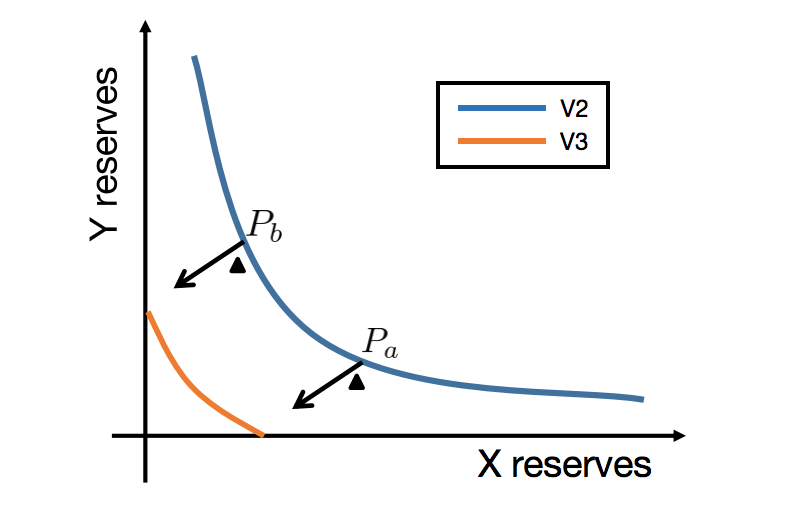
\includegraphics[width=0.6\textwidth]{krivulja.png}
        %\caption{Krivulja}
\end{figure}



% #Pri koncentrirani likvidnosti, se lahko ponudniki likvidnosti odločijo, da bodo svoj denar skoncentrirali na določen cenovni razpon. Ponudniki likvidnosti zaslužijo več provizij za manj kapitala, saj je njihov denar skoncentriran na območju, kjer se odvija največ trgovalnih dejavnosti.V primeru, da se cena premakne izven izbranega območja, likvidnost ponudnika ni več aktivna in provizij ne prejemajo dokler se cena ne pomakne nazaj v cenovno območje, ki ga je izbral. 
% #Ta pristop povečuje kapitalsko učinkovitost, saj so vsa sredstva razporejena tam, kjer je trgovanje najvrjetnejše.



% #V sistemu Uniswap V3 lahko ponudniki likvidnosti koncentrirajo svoj kapital znotraj cenovnih razponov po meri, kar zagotavlja več likvidnosti po želenih cenah. Pri tem oblikujejo individualizirane cenovne krivulje, ki odražajo njihove preference. Ponudniki likvidnosti lahko združijo poljubno število različnih koncentriranih pozicij znotraj enega sklada.
% #S koncentriranjem njihove likvidnosti lahko ponudniki nudijo enako likvidnost kot V2 v določenem cenovnem območju z manj tveganega kapitala. Namesto, da zagotavljajo enako likvidnost, kot ponudniki v V2, lahko ponudniki likvidnosti v V3 ponudijo več likvidnosti z enakim kapitalom, za kar pa morajo prevzeti več cenovnega tvegnja (impermanent loss), in s tem ponujajo več trgovanja in zaslužijo več provizij.
% #V primeru, da se tržne cene premaknejo izven določenega območja ponudnika likvidnosti, je njihova likvidnost izvzeta iz likvidnostnega bazena in ponudnik ne prejema provizij, dokler se tržne cene ne vrnejo v specificirano območje. 


Zaradi koncentrirane likvidnosti ponidnikove likvidnostne pozicije niso več zamenljive in v protokolu niso več predstavljene kot ETC-20 token. Namesto tega so prestavljene kot NTF-ji. 


\subsubsection{Prilagodiljive provizije}
Uniswap V3 je uvedel prilagoljive provizije, kjer lahko ponudnik likvidnosti določi provizijo, glede na ugotovljeno tveganje para tokenov, za katerega zagotavlja likvidnost. Na podlagi volatilnosti para lahko izbira med provizijami v višini 0.05 \%, 0.3 \% in 1 \%. 




\subsection{Primerjava}

Čeprav imata tako V2 kot V3 svoje prednosti, je temeljna razlika v kapitalski učinkovitosti in potencialnih donosih za ponudnike likvidnosti. Uvedba koncentrirane likvidnosti v različici V3 je spremenila način zagotavljanja likvidnosti v sistemu Uniswap in ponudila možnost veliko večjih donosov na naložbe. Medtem ko ima V2 enostaven pristop k zagotavljanju likvidnosti, je V3 kompleknejša in zahteva globlje razumevanje tržne dinamike in gibanja cen. Ponudniki likvidnosti morajo aktivno upravljati svoje pozicije in prilagajati cenovna območja za svojo likvidnost. 

%Vir: \url{https://medium.com/@92CLUB.ETH/uniswap-v2-vs-uniswap-v3-evolution-of-a-decentralized-exchange-df0771dce609}

\end{document}

